%Centralizar verticalmente.
\newenvironment{midpage}{\vspace*{\fill}}{\vspace*{\fill}}
%Centralizar horizontalmente.
\newenvironment{midline}{\hspace*{\fill}}{\hspace*{\fill}}
\documentclass[12pts]{article}
\usepackage[utf8]{inputenc}
%Pacote para colocar cor no código.
\usepackage{color}
\definecolor{light-gray}{gray}{0.95}
%Pacote para inserir código.
\usepackage{listings}
\lstset{
    numbers=left,
    tabsize=2,
    backgroundcolor=\color{light-gray},
}\title{
	Prática de Eletrônica Digital 1 - (119466)
	\singlespacing
		Turma E (Unb - Gama)
	\singlespacing
	\begin{midpage}
	\begin {large}
		Projeto Final
		\singlespace
		Gerador de números aleatórios
	\end {large}
	\end{midpage}
}
\date{Novembro 16, 2016}
\usepackage{indentfirst}
\usepackage{setspace}
\usepackage{verbatim}
\usepackage[pdftex]{hyperref}
\usepackage{graphicx}
\begin{document}
\maketitle	
%\vspace{100 mm}
\begin{center}

\begin{tabular}{|c|l|r|}
\hline
Nome & Matrícula & Assinatura\\
\hline

Arthur Temporim & 14/0016759 & \\
\hline	
Eduardo Nunes & 14/0056189 & \\

\hline	
\end{tabular}

\end{center}


\newpage

\section{Sumário}

\begin{itemize}
	\item Introdução
	\singlespacing
	\item Descrição do projeto
	\singlespacing
	\item Discussão
	\singlespacing
	\item Conclusões 
	\singlespacing
	\item Referências Bibliograficas
	\singlespacing
	%\item Diagramas esquemáticos
\end{itemize}

\newpage


\section{Introdução}
\iffalse
Introdução, indicando a delimitação do tema, apresentando a justificativa descrevendo o propósito do relatório.
\fi

	Neste relatório é apresentado o resultado do projeto de um Gerador de números aleatórios para a disciplina de prática de eletrônica digital 1. São apresentados o funcionamento do projeto, com representações em imagens, as especificações das entradas e saídas utilizadas no kit BASYS3, juntamente, com o arquivo de restrição, o código VHDL assimm como diagrama do circuito. 


\section{Projeto}
\iffalse
Parte Experimental, descrevendo os passos realizados, dificuldades e soluções para os problemas encontrados. Aqui, deve-se apresentar uma descrição dos resultados encontrados em forma de figuras, gráficos e tabelas.
\fi

\singlespacing

\subsection{Objetivo}
	O objetivo deste projeto é implementar um gerador de números aleatórios de 2 elevado a m, menos 1 estados. Um gerador de números aleatórios é um algoritmo que gera uma sequência de números, os quais são aproximadamente independentes um dos outros. A saída da maioria dos geradores de números
aleatórios não é verdadeiramente aleatória, ela somente aproxima algumas das propriedades dos
números aleatórios.
		
\subsection{Funcionamento}
	O projeto funciona da seguinte forma: O primeiro passo é transformar o valor binário do grupo, no caso o k (variável que seleciona um grupo de até 16 bits). Logo, em seguida a opção de ativar o modo de geração de um número, opção de nível baixo, ou de validar a geração, nível alto. Supondo se que foi selecionado a opção de gerar um número aleatório, então o projeto aplica a geração aleatória. Em seguida, da o shift nos bits de borda de subida, deslocando assim os bit que pode ser com base em um clock ou de uma chave seletora. Este faz a verificação de se os 4 últimos digitos forem iguais ao valor a variavél que seleciona o valor, no caso S. Então, há a contagem de quantas vezes o valor de S aparece no vetor. Logo em seguida, o resultado é exposto no display.

\clearpage
\subsection{Código VHDL}
\lstinputlisting[language=vhdl]{projeto/Main.vhd}

\clearpage
\subsection{Diagrama do circuito}
\begin{figure}[!htb]
  \centering
  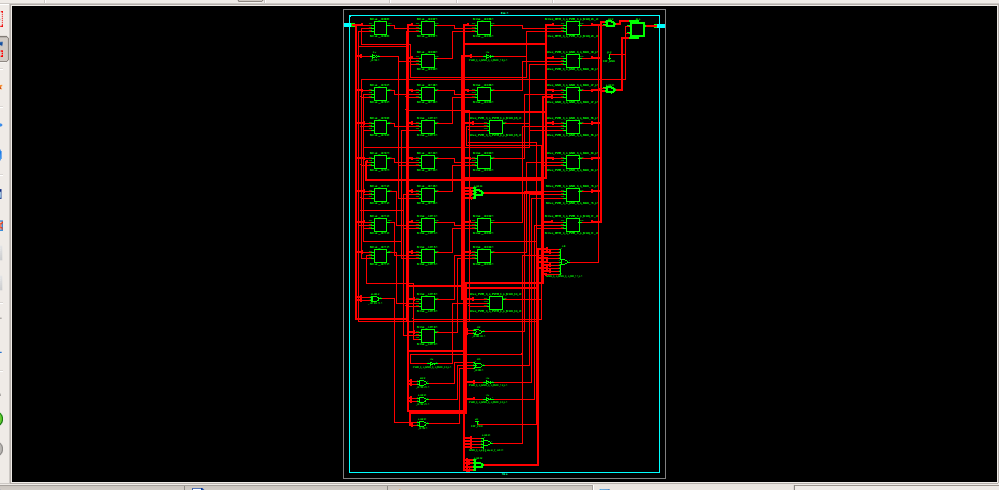
\includegraphics[scale=0.45]{imagens/circuito}
  \caption{Diagrama do circuito de um gerador de números aleatórios}	
  \label{figRotulo}
\end{figure}

\newpage

\subsection{Resultados}

\subsection{Metodologia de testes}


\section{Discussão}
\iffalse
Discussão sobre os resultados encontrados, comentando detalhadamente as medições realizadas e dando a devida interpretação destas, informando se os objetivos da experimento foram alcançados. Esta é uma das partes mais importantes do relatório: aqui, há oportunidade para expressar os conhecimentos adquiridos na prática e fazer a interrelação com os fundamentos teóricos.
\fi

        Neste projeto final, os objetivos foram atingidos havendo a geração de números pseudo-aleatórios. 

\section{Conclusões}
\iffalse
Conclusões, mostrando os êxitos e eventuais problemas encontrados na realização do experimento, indicando as limitações, apresentando recomendações e/ou sugestões.
\fi

Com a realização deste experimento foi possível adquirir conhecimento a respeito de mais funções do VHDL que facilitam o trabalho do desenvolvedor assim como de projetar um circuito na FPGA utilizando se de mais recursos e ganhar bastante conhecimento a respeito da geração de números aletórios, que consiste em conhecer a existencia outras formas e métodos de se fazer a geração e verificação destes. 

\section{Referências Bibliográficas}
\iffalse
Referencias Bibliográficas, relacionadas e citadas de acordo com as normas da ABNT.
\fi
Prática de Eletrônica Digital I 2016.2 professores Henrique Marra Taira Menegaz,Leonardo Aguayo, Lourdes Mattos Brasil, Marcus Vinícius Chaffim Costa, Mariana Costa Bernardes Matias. UnB - FGA Agosto de 2015.

\iffalse
\section{Diagramas Esquemáticos}
Diagramas Esquemáticos. Todos os diagramas devem ser inseridos ao final do relatório em páginas separadas do texto, indicando a identificação do circuito, autor, revisor, versão e datas relevantes.
\fi
\newpage

\end{document}
